\chapter{Technical Background}
\label{sec:state}

% Hier werden zwei wesentliche Aufgaben erledigt:

% 1. Der Leser muß alles beigebracht bekommen, was er zum Verständnis
% der späteren Kapitel braucht. Insbesondere sind in unserem Fach die
% Systemvoraussetzungen zu klären, die man später benutzt. Zulässig ist
% auch, daß man hier auf Tutorials oder Ähnliches verweist, die hier auf
% dem Netz zugänglich sind.

% 2. Es muß klar werden, was anderswo zu diesem Problem gearbeitet
% wird. Insbesondere sollen natürlich die Lücken der anderen klar
% werden. Warum ist die eigene Arbeit, der eigene Ansatz wichtig, um
% hier den Stand der Technik weiterzubringen? Dieses Kapitel wird von
% vielen Lesern übergangen (nicht aber vom Gutachter ;-), auch später
% bei Veröffentlichungen ist "Related Work" eine wichtige Sache.

% Viele Leser stellen dann später fest, daß sie einige der Grundlagen
% doch brauchen und blättern zurück. Deshalb ist es gut,
% Rückwärtsverweise in späteren Kapiteln zu haben, und zwar so, daß man
% die Abschnitte, auf die verwiesen wird, auch für sich lesen
% kann. Diese Kapitel kann relativ lang werden, je größer der Kontext
% der Arbeit, desto länger. Es lohnt sich auch! Den Text kann man unter
% Umständen wiederverwenden, indem man ihn als "Tutorial" zu einem
% Gebiet auch dem Netz zugänglich macht.

% Dadurch gewinnt man manchmal wertvolle Hinweise von Kollegen. Dieses
% Kapitel wird in der Regel zuerst geschrieben und ist das Einfachste
% (oder das Schwerste weil erste).

% Background Warum ist das Thema wichtig?
% Was ist das Smart Grid -> mit Background verknüpfen
% Vor, Nachteile vom Smart Grid?
% Was sind Smart Meter
% Warum sind Smart Meter Privacy relevant?
% DC-Netze einführen
% Related Work: Welche andere Verfahren gibt es?
% Vllt erklärung regeln vom BSI

This section introduces an overview of the basic concepts for this work. Therefore, the key components of the smart grid are explained, what structural changes and what challenges the smart grid will bring.
In addition, this chapter discusses the current state of research.\\

\section{Smart Grid}
The original energy network was mainly considered as a transmission system to send electricity from the generators via a elongated network of cables and transformers to the consumers.% vllt hier noch schreiben, dass es erneuerbare Energien wegen der Klimakriese gibt
Instead of a few electricity producers (e.g. nuclear power plants, coal-fired power plants), which were responsible for a large part of the electricity generation, there are now many smaller producers (e.g. wind turbines). %However, renewable power generation is often dependent on external environmental influences. Therefore, smart meters have been widely introduced in households to ensure that the smart grid is stable despite fluctuations in power generation.
However, renewable power generation is often dependent on external environmental factors. In order for the smart grid to be stable despite fluctuations in power generation, smart meters have been introduced.
This enables the electricity provider to receive the electricity consumption of a household every 15 minutes. It offers the possibility to get more easily the current electricity demand from the consumers. Previously, the current electricity demand was simulated from load forecasting models. If the demand should increase spontaneously, peaker plants, mainly consisting of coal-fired power plants, would be turned on to quickly meet this demand. This is costly and environmentally unfriendly. 
Since then, structural changes have been made to optimize the energy grid and make it more intelligent by exchanging information in near-real-time. This allows the demand to be matched to the available supply. The fundamental component of the smart grid are the smart meters, which were already mentioned. They which will be discussed in more detail in the next section.(Quelle:Smart Grid Communications)(Privacy Survey2013)

\section{Smart Meter}
Smart meters are the key component in a smart grid. A smart meter is an electricity meter that has an interface to the Internet. It enables two-way communication between the control center and the meter. This is also called Advanced Metering Infrastructure (AMI). Two-way communication improves the quality of the power grid and makes it possible to offer services that would not be feasible without a smart meter. For example it's now practicable to detect power outages.%hier nochmal was ändern.
As a result, the power grid operator can detect power failures on its own. Previously, the operator was dependent on customer calls to detect power outages. Another new feature is detailed monitoring of power flows at the smart meter. Before, power flows could only be measured up to substations. This new function enables electricity network operators to quickly detect changes in consumption behavior and react to them without having to use peaker plants, which are costly and environmentally unfriendly. Depending on the setting, smart meters can send electricity consumption to the electricity provider at least every 15 minutes. In combination with the consumption of all users and the current electricity supply, a better price can be achieved. This is also called real-time pricing. So not only can the customer be offered a better electricity contract, in addition the meters no longer have to be read at home by a technician from the electricity provider. This makes billing easier for customers and electricity providers. Furthermore, customers can also check their current electricity consumption via the interfaces provided by the smart meter in order to analyze their own behavior and to reduce their consumption. (Privacy-Aware Smart Metering)
%Thus, the end user can analyze his own consumption behavior in order to reduce his own electricity consumption.
\section{Smart Meter Privacy}
The main advantage of the smart grid is the communication between the consumers and the energy suppliers. It is precisely this communication that solves a lot of structural problems in today's energy system. However, sending user information every 15 minutes allows for new methods that can be used to create accurate behavioral analyses in one's own home. Sending private electricity consumption data is therefore very sensitive information and must to be protected. This is not an easy task, because on the one hand the electricity consumption must be protected and anonymized, and on the other hand the billing and costs must be clearly assignable to a person. In the following paragraphs, we will describe how simple behavioral analyses are generated by electricity consumption. Subsequently, solutions to Metering for Billing and Metering for Operations will be presented, which have been discussed in the scientific community so far.(Privacy-Aware Smart Metering) 
\subsection{Non-intrusive load monitoring} 

Interpreting power consumption with the intent of identifying devices in the home is called non-intrusive load monitoring (NILM). George Hart and Fred Schweppe were the first to develop non-intrusive load monitors in 1985 and connect them to electricity meters. They were able to record the current power consumption up to every 5 seconds. Then they did the following steps to identify appliances in a household:
\begin{enumerate}
\item Edge Detection:\\
Look for sharply rising or steeply falling edges in the stored electricity consumption. These edges indicate that a device may have been switched on or off at that moment.
\item Cluster Analysis:\\ 
The events of steeply rising or steeply falling edges are saved. These events are then visualized in a graph with the following characteristics. Each event is ordered according to how much power was consumed or how much power was 	``released'' from the device (e.g. when it was switched off).
Essentially, a cluster analysis is then applied to the diagram and each  cluster represents a household appliance.
\item Appliance Model Construction\\
Since different household appliances have been determined by the clusters, appliance models can now be constructed. In this step, different states in which an appliance can be in, are found based on the different power consumption. An example of how the result of a appliance model looks like can be seen in Figure 2.1.


\begin{figure}[tbp]
  \centering
  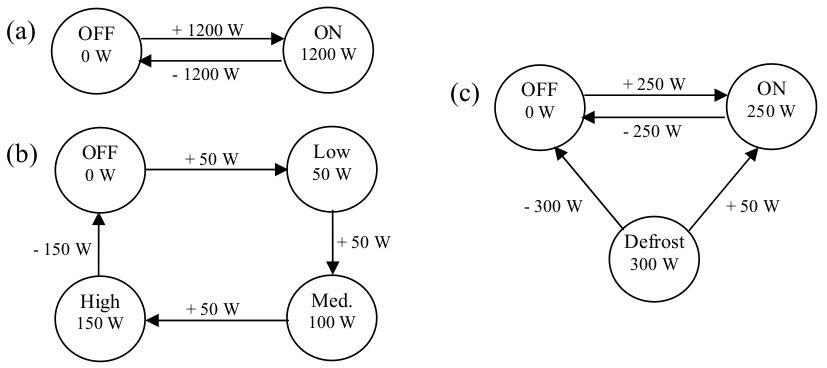
\includegraphics[width=1\textwidth]{images/Appliance_Model.png}
  \caption[Short description]{An example of a NILM analysis.}
  \label{fig:Appliance_Model}
\end{figure}
\item Behavior Analysis:\\
Once the majority of the household appliances have been identified, the behaviors of people in the household can be analyzed. In real time, it is possible to track the use of devices, since individual signals can be identified as they occur and do not need to be reconstructed anymore.
At this point, several approaches can be taken to provide behavioral analysis. A common approach is to track how long a device has been in use and create statistics on how each device has been used. A daily analysis can be viewed in Figure 2.2.
\item Appliance Saving:\\
The last approach is to name the household appliances found(washing machine, etc.) and store them in a database. So that in the case of a further household analysis, it is possible to fall back on appliances that have already been found.
\end{enumerate}
The founder of NILM G. W. Hart himself said in 1989: ``Specifically, I recommend that legal restrictions be enacted or clarified so that electric power usage is considered as private as any phone conversation.''(Residential Energy Monitoring)
Hence, there is a need for a privacy-preserving solution for smart meters.
Although the original NILM approach measured power consumption every 5 seconds, there are now methods to identify household appliances when power consumption is measured every 15 minutes.(A Neuron Nets Based)
\begin{figure}[tbp]
  \centering
  \includegraphics[width=1\textwidth]{images/nilm.png}
  \caption[Short description]{An example day of a NILM analysis.}
  \label{fig:Nilm}
\end{figure}
\subsection{Metering for Operations}
\\
The paragraph deals with solutions for Metering for Operations, which has been previously discussed in other scientific works. At Metering for Operations, there is currently no established consensus on a solution. Various technical proposals have already been presented in scientific papers, but there is a lack of uniform criteria and often different conditions are set for the power grid. One reason for this could be that smart grids are realized differently in other countries. In the following, the different approaches are divided into categories and presented conceptually.\\
\\
\textbf{Anonymization or Pseudonymization
Without Aggregation}
\\
\\
This approach describes the removal of smart information that allows identification. Identifiable information can also be replaced by pseudonyms. Solutions with trusted third parties are often used in this case. A trusted third party usually acts as an intermediary between the customer and the power grid provider. The trusted third party must be acknowledged by all participants and take a neutral position. In practice, however, this is difficult to achieve because the trusted third party is often hired as a service provider by the electricity supplier and is therefore also paid by the supplier.\\
\\
In the paper "A privacy-preserving Concept for Smart Grids" by Petrlic[quelle], a trusted third party is used as an intermediary. In the proposal, a smart meter communicates with a trusted third party. Certificates formed with a public key infrastructure can be used to verify and validate information flows from smart meters at the TTP. As soon as the Trusted Third Party has checked the correctness of the smart meter information, it can pseudonomize/anonymize all the necessary information. Only then is the further processed anonymized information forwarded to the electricity provider by the TTP in encrypted form. This means that the electricity provider cannot assign individual electricity consumption to its customers. With this procedure, smart meters can be anonymized. 
However, if it is possible for an attacker to record the data traffic between the smart meter and the TTP, then the attacker could forward the time stamps and smart meter identification to the electricity provider. Using these two pieces of information, the electricity provider could at least gain some insight, since it would be possible to match when information is sent to the TTP and when it is received by electricity provider.(Privacy-Aware Smart Metering) \\
\\
\textbf{Aggregation with Trusted Third Parties}
\\
\\
In the attack just described, the electricity provider tries to link two events. One is the arrival of the message at the TTP and the other is the arrival of the message at the provider itself. One way to prevent this attack is aggregation. In this case, the smart meter sends its electricity consumption to the TTP. Certificates are also sent from the smart meter so that the TTP can check the information for correctness and authenticity. Instead of forwarding the information to the electricity provider, the TTP waits until all smart meters have sent their data for which the TTP is responsible. This data is all added up and a message is sent from the TTP to the electricity provider with the total electricity consumption of all smart meters. From the aggregated value, it is not possible to extract an individual smart meter's electricity consumption, which is why the electricity provider cannot filter out information about individual customers.(A Privacy Model for Smart Metering)\\
Homomorphic encryption approaches also fall into this category. Homomorphic encryption algorithms allow simple operations such as addition and multiplication to be performed on the encrypted messages.  In some homomorphic encryption schemes, only addition OR multiplication are supported. These are then called partial homomorphic encryption.
There are also bihomorphic encryption approaches. Here not only the operations on the ciphertexts are homomorphic, but also the operations on the keys. This means that if a plaintext a is encrypted with the key x and a plaintext b is encrypted with the key z, that one can decrypt the ciphertexts enc(a+b) with the keys x+z. A bihomomorphic encryption approach with TTP has been proposed by Vetter et al.[quelle] In this case, the TTP acts as the key authority. This means that it creates all cryptographic keys and forwards them to the smart meter, which is then used for further communication with a central store. The smart meter encrypts its data and sends it to the central storage. The central storage also stores the incoming data in encrypted form, so that no unencrypted data can be found on the storage. In addition, the central storage has no access to the keys and thus has no way to decrypt the information or access meaningful data.



\todo{write state}

\cleardoublepage

%%% Local Variables:
%%% TeX-master: "diplom"
%%% End:
